% =============================================================================
% SpatialLens Assist --- CS131 Final Report
% -----------------------------------------------------------------------------
% Compile with: latexmk -pdf main.tex
% Figures live in figures/ and figures/final/; tables in tables/.
% =============================================================================

\documentclass[10pt,twocolumn,letterpaper]{article}

\usepackage[margin=0.55in,top=0.5in,bottom=0.55in]{geometry}
\usepackage{graphicx}
\graphicspath{{figures/}{figures/final/}}
\usepackage{booktabs}
\usepackage{caption}
\usepackage{subcaption}
\usepackage{enumitem}
\usepackage{hyperref}
\usepackage{url}
\usepackage{amsmath}
\usepackage{amssymb}
\usepackage{xcolor}
\usepackage{colortbl}
\usepackage{array}
\usepackage{makecell}
\usepackage[expansion=false,protrusion=false]{microtype}
\usepackage{siunitx}
\sisetup{detect-all,group-separator={,}}
\usepackage{tikz}
\usetikzlibrary{shapes.geometric,arrows.meta,positioning,calc,fit,backgrounds}
\usepackage[capitalize,noabbrev]{cleveref}

% Architecture-diagram palette + text macros.
\definecolor{cInput}{HTML}{ECEFF1}
\definecolor{cDet}{HTML}{D7E3F0}
\definecolor{cTrack}{HTML}{FBE2C4}
\definecolor{cMotion}{HTML}{D8ECD9}
\definecolor{cClf}{HTML}{E7DCF0}
\definecolor{cContrib}{HTML}{E8820C}
\newcommand{\hdr}[1]{{\sffamily\bfseries\footnotesize #1}}
\newcommand{\subt}[1]{{\sffamily\scriptsize\textcolor{black!75}{#1}}}

% Relax conservative float-packing defaults so wide (table*/figure*)
% floats can share a page top instead of spilling onto a dedicated
% float page.
\setcounter{topnumber}{3}
\setcounter{dbltopnumber}{3}
\setcounter{totalnumber}{5}
\renewcommand{\topfraction}{0.95}
\renewcommand{\dbltopfraction}{0.95}
\renewcommand{\bottomfraction}{0.4}
\renewcommand{\textfraction}{0.05}
\renewcommand{\floatpagefraction}{0.7}
\renewcommand{\dblfloatpagefraction}{0.7}

\hypersetup{colorlinks=true,urlcolor=blue!60!black,linkcolor=black,citecolor=blue!60!black}
\captionsetup{font=small,labelfont=bf,skip=3pt}
\setlist{nosep,leftmargin=*}
\setlength{\columnsep}{0.25in}
\pagestyle{empty}

\title{\vspace{-2em}\Large\bfseries SpatialLens Assist: Motion-Aware Hazard\\Detection
for Campus Navigation from Low-FPS Egocentric Video}
\author{
  Diego Sanchez \\
  Stanford University \\
  \texttt{dsanh14@stanford.edu}
}
\date{}

\begin{document}
\twocolumn[
  \begin{@twocolumnfalse}
    \maketitle
    \vspace{-2.5em}
    \vspace{0.5em}
    \begin{abstract}
      \noindent
      An object detector tells a blind pedestrian \emph{what} is
      nearby, but not whether it is closing, crossing, or simply
      present. We ask whether a small, interpretable set of motion
      cues---bounding-box growth, centroid displacement, optical flow,
      and ego-motion compensation---can recover useful hazard labels
      from low-fps handheld campus video, without training a learned
      trajectory model. We present \textbf{SpatialLens Assist}, an
      end-to-end CPU pipeline that converts short ($\sim$10\,s)
      walkway clips into per-track motion-aware alerts over six
      classes (\texttt{approaching}, \texttt{crossing\_LTR},
      \texttt{crossing\_RTL}, \texttt{moving\_away}, \texttt{static},
      \texttt{uncertain}). The system pairs YOLOv8n with an
      IoU+centroid tracker, ego-motion-compensated Farneback flow and
      frame differencing, per-track motion aggregates, and a transparent
      rule cascade that emits a natural-language evidence string and
      treats \texttt{uncertain} as a first-class abstention rather
      than a guess. On 11 controlled walkway videos (61 manually
      labelled tracks), the system reaches \textbf{82.5\%} overall
      accuracy on 57 evaluated track--label pairs and \textbf{93.3\%}
      on the 30 tracks with at least three frames, with approaching
      precision/recall \textbf{0.95/0.88}---the safety-asymmetric
      regime an alert layer needs. Ablations show the largest gain
      comes from tracker continuity (\(+\)6.2\,pts from
      appearance-gated re-identification, \(+\)3.5\,pts each from
      two short-track salvage rules), and ByteTrack is a negative
      result on this sparse 2\,fps regime (32.8\%). The dominant
      failure mode is conservative abstention from tracker
      fragmentation, not dangerous mislabelling: \emph{no}
      \texttt{approaching}\(\leftrightarrow\)\texttt{moving\_away}
      confusion occurs.
    \end{abstract}
    \vspace{1em}
  \end{@twocolumnfalse}
]

% --------------------------------------------------------------------------
\section{Introduction}
% --------------------------------------------------------------------------
A bicycle parked against a wall and a bicycle bearing down on the
camera are both detected as ``bicycle, 0.86.'' For a sighted user the
wider visual context carries the intent; for a blind or low-vision
pedestrian relying on an assistive device such as Seeing
AI~\cite{seeingai} or a wearable navigation aid~\cite{poggi2016}, that
context is exactly what is missing. The safety-critical signal is not
the class label but the \emph{motion}: whether the agent is closing,
crossing the path, or merely present.

We frame motion-aware hazard detection as \emph{per-track
classification}: given a $\sim$10\,s phone clip sampled at 2\,fps,
decide for each tracked object whether it is approaching, crossing
left-to-right, crossing right-to-left, moving away, static, or
explicitly \texttt{uncertain}. Three properties drive the design:
(i)~\textbf{explainability} -- every prediction carries a textual
evidence string; (ii)~\textbf{calibrated abstention} -- short tracks
do not bluff, so \texttt{uncertain} is a first-class output with a
sub-reason; (iii)~\textbf{reproducibility on CPU} -- the full pipeline
runs in $\sim$4\,min on a GPU-less Mac and the 61-track labelled set is
committed.

\noindent\textbf{Summary.} On 11 controlled walkway videos and 61
labelled tracks the system reaches 82.5\% accuracy on 57 matched tracks
(93.3\% on the 30 decidable tracks with $\ge$3 frames);
\texttt{approaching} reaches 0.95\,/\,0.88 precision/recall and no
\texttt{approaching}$\leftrightarrow$\texttt{moving\_away} confusion is
observed. Isolated ablations attribute the dominant gain to track
continuity rather than classifier complexity: appearance-gated
re-identification contributes 6.2\,pts and the two 2-frame salvage
rules 3.5\,pts each, while ByteTrack on 2\,fps offline footage drops
to 32.8\% -- a useful negative result.

\noindent\textbf{Contributions.} (\textbf{C1})~a CPU-only offline
egocentric pipeline for motion-aware campus hazard alerts;
(\textbf{C2})~ego-motion-compensated motion features (median-subtracted
Farneback flow + ECC-aligned frame differencing) appropriate to
handheld low-fps footage; (\textbf{C3})~an interpretable hazard rule
cascade with natural-language evidence strings, conservative
abstention, and a trajectory-reversal heuristic for
``approached-then-turned-away'' tracks; (\textbf{C4})~a 61-track
evaluation set with two reporting denominators and a fully scripted
ablation suite; (\textbf{C5})~empirical evidence that tracking
continuity dominates classifier sophistication in this regime, and
that ByteTrack is poorly matched to sparse offline footage.

% --------------------------------------------------------------------------
\section{Related Work}
% --------------------------------------------------------------------------

\noindent\textbf{Detection and tracking.} YOLOv8~\cite{ultralytics} is
a fixed COCO-class front-end. SORT~\cite{sort} and
ByteTrack~\cite{bytetrack} are strong online baselines but assume
near-continuous per-frame detections from a Kalman model; on our
2\,fps footage ByteTrack (via
\texttt{supervision}~\cite{supervision}) drops 51\% of detections,
motivating a transparent per-class IoU+centroid matcher with explicit
gap buffer plus a separate appearance-gated re-ID pass tailored to
sparse sampling. Assistive tools such as
Seeing AI~\cite{seeingai} and academic prototypes~\cite{poggi2016}
expose object \emph{identity} but rarely \emph{motion intent}.

\noindent\textbf{Trajectory prediction vs.\ past-motion classification.}
Trajectron++~\cite{trajectronpp} and
Social-STGCNN~\cite{socialstgcnn} forecast \emph{future} positions
over 4--8\,s from high-fps tracks with map context, requiring
thousands of training trajectories. We solve the strictly easier
problem of classifying the \emph{past} motion of a single track into
six safety-relevant categories from $\sim$10 sampled frames, choosing
an alert plus evidence string over a future-position
distribution -- a deliberate scope choice driven by the no-training-data
setting and the explainability/abstention requirements of an
assistive interface. Classical Farneback flow~\cite{farneback} and
ECC alignment~\cite{ecc} support the CPU-only constraint;
median-flow subtraction compensates for the camera pan that
otherwise inflates apparent motion of every static object.

% --------------------------------------------------------------------------
\section{Method}
\label{sec:method}
% --------------------------------------------------------------------------

\begin{figure*}[t]
  \centering
  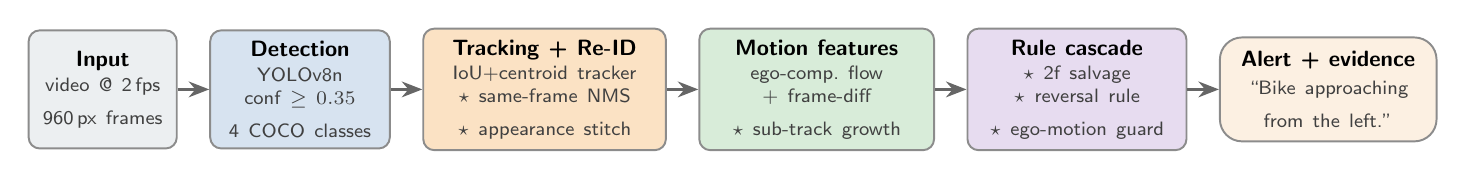
\begin{tikzpicture}[
    font=\sffamily,
    stage/.style={rounded corners=4pt, draw=black!45, line width=0.7pt,
                  align=center, minimum height=15mm, inner sep=4pt},
    flow/.style={-{Stealth[length=2.6mm,width=2mm]}, line width=1.1pt, draw=black!60},
  ]
  \node[stage, fill=cInput, text width=16mm] (inp)
    {\hdr{Input}\\[1pt]\subt{video @ 2\,fps\\960\,px frames}};
  \node[stage, fill=cDet, right=4mm of inp, text width=20mm] (det)
    {\hdr{Detection}\\[1pt]\subt{YOLOv8n\\conf $\geq 0.35$\\4 COCO classes}};
  \node[stage, fill=cTrack, right=4mm of det, text width=28mm] (trk)
    {\hdr{Tracking + Re-ID}\\[1pt]\subt{IoU+centroid tracker\\$\star$ same-frame NMS\\$\star$ appearance stitch}};
  \node[stage, fill=cMotion, right=4mm of trk, text width=27mm] (mot)
    {\hdr{Motion features}\\[1pt]\subt{ego-comp.\ flow\\+ frame-diff\\$\star$ sub-track growth}};
  \node[stage, fill=cClf, right=4mm of mot, text width=25mm] (clf)
    {\hdr{Rule cascade}\\[1pt]\subt{$\star$ 2f salvage\\$\star$ reversal rule\\$\star$ ego-motion guard}};
  \node[draw=black!45, rounded corners=8pt, fill=cContrib!12, line width=0.7pt,
        right=4mm of clf, text width=24mm, align=center, inner sep=5pt] (out)
    {\hdr{Alert + evidence}\\[2pt]\subt{``Bike approaching\\from the left.''}};
  \draw[flow] (inp) -- (det);
  \draw[flow] (det) -- (trk);
  \draw[flow] (trk) -- (mot);
  \draw[flow] (mot) -- (clf);
  \draw[flow] (clf) -- (out);
  \end{tikzpicture}
  \caption{End-to-end SpatialLens pipeline. The detector is
  off-the-shelf; \textcolor{cContrib}{$\star$} marks the four
  contributions evaluated in \Cref{sec:results} (same-frame NMS,
  appearance-gated re-ID, sub-track growth features, and the
  rule-cascade salvage/guard rules). Every prediction carries a
  natural-language \emph{evidence string} that the alert layer quotes,
  and \texttt{uncertain} is a first-class output with a sub-reason
  rather than a fall-through default.}
  \label{fig:pipeline}
\end{figure*}

The pipeline (\Cref{fig:pipeline}) has six stages. We summarise each,
focusing on the four non-obvious design decisions.

\subsection{Frames, detection, base tracking}
Videos are sampled at 2\,fps, resized to 960\,px wide.
YOLOv8n~\cite{ultralytics} emits per-frame detections at
conf~$\ge\!0.35$. A per-class IoU+centroid tracker -- IoU association
in the spirit of SORT~\cite{sort}, but augmented with a centroid term
and an explicit gap buffer for the sparse-sampling regime -- matches
greedily by
$s_{dt}=0.7\cdot\textrm{IoU}(d,t)+0.3\cdot(1-\hat d_{dt})$ with a
\texttt{max\_frame\_gap} buffer so a track survives 1--2 missed
detections.

\subsection{Motion features with ego-motion compensation}
\label{sec:motion}
Handheld panning makes every static object appear to move. We
compensate two ways: \textbf{flow} -- Farneback dense
flow~\cite{farneback} between frames, minus the per-frame median flow
vector (background-dominated), giving per-bbox
$(\textrm{flow\_dx},\textrm{flow\_dy},\textrm{flow\_mag})$
relative to the scene; \textbf{frame diff} -- align the previous
frame to the current with ECC alignment~\cite{ecc}
(\texttt{cv2.findTransformECC}, translation) before differencing. Per-track aggregates: start-to-end
growth $r=(A_{\textrm{end}}-A_{\textrm{start}})/A_{\textrm{start}}$,
total $\Delta\!c_x$, mean flow magnitude, plus two sub-track signals
for reversal detection -- second-half growth $r_{1/2}$ and peak-area
ratio $\rho=\max_t A_t / A_{\textrm{end}}$.

\subsection{Conservative fragment re-identification}
\label{sec:reid}
At 2\,fps a fast-crossing object moves up to 350\,px between samples,
so the tracker fragments single objects. A post-tracker cleanup
applies (i)~\textbf{same-frame NMS} (drop overlapping same-class
detections at IoU~$\ge\!0.5$) and (ii)~\textbf{appearance-gated
stitching}: merge tracks $B\!\to\!A$ only if \emph{all} of same class,
\emph{both tracks $=$ 1 frame}, gap~$\le\!2$, centroid distance
$\le\!0.45$\,diag, area ratio $\le\!5$, and HSV $(H,S)$ histogram
correlation $\ge\!0.45$. The 1-frame constraint protects multi-frame
tracks from being absorbed by fragments -- an aggressive variant
broke seven correct tracks (\cref{sec:bytetrack}).
\texttt{src/track\_reid.py} keeps cleanup separable for ablation.

\subsection{Rule-cascade hazard classifier}
\label{sec:classifier}

The classifier resolves the label by a priority cascade, each branch
carrying its own evidence template ($r$: bbox-growth ratio;
$\rho$: peak/end area ratio; $r_{1/2}$: second-half growth):
\textbf{(1)~Short-track salvage} ($n\!=\!2$): strong lateral
$|\textrm{dx\_norm}|\!>\!0.30\to$crossing, else strong approach
($r\!>\!0.7$, downward flow)$\to$\texttt{approaching}, else
\texttt{uncertain}. \textbf{(2)~Static} if $n\!\ge\!3$ and no motion.
\textbf{(3)~Moving-away} if $r\!<\!-0.15$, or the \emph{soft} variant
($-0.15\!<\!r\!<\!-0.03$ with sub-strong lateral motion read as
ego-motion drift). \textbf{(4)~Trajectory reversal} ($n\!\ge\!6$,
$r\!>\!0.3$, $\rho\!>\!1.5$, $r_{1/2}\!<\!-0.20$)$\to$
\texttt{moving\_away} for the ``approached then turned away'' case.
\textbf{(5)~Strong crossing} ($|\textrm{dx\_norm}|\!>\!0.50$)
overrides approach. \textbf{(6)~Approaching} if
$\textrm{approach\_score}\!\ge\!0.55$ and ($r\!>\!0.15$ or the
slow-approach allowance $r\!>\!0$ with score $\ge\!0.65$).
\textbf{(7)~Crossing} if $|\textrm{dx\_norm}|\!>\!0.08$, $r\!\le\!0.15$.
\textbf{(8)~Uncertain} fall-through, tagged with the closest-missed
sub-reason (\texttt{near\_approaching}, \texttt{low\_signal}, \dots)
quoted in the evidence string.

\noindent The \emph{approach score} is a fixed-weight blend
$0.45\cdot s_{\textrm{growth}}+0.25\cdot s_{\textrm{center}}+
0.20\cdot s_{\textrm{fd}}+0.10\cdot s_{\textrm{flow}}$ of four
normalised cues (bbox growth, centroid motion toward image
center/lower half, frame-diff overlap, and flow magnitude).

\subsection{Alert generation and explainability}
Every prediction carries a templated \emph{evidence string} quoting
the feature values that triggered the cascade branch
(e.g.\ ``\texttt{classified as approaching because bbox grew by 11.42
and approach\_score = 1.00; centroid moved toward image
center/lower half; flow\_mag = 17.26}''); for abstentions the string
names the sub-reason. Tracks with $<\!3$ frames are not forced into
a motion class -- treating uncertainty as safety-preserving
abstention. A 4-frame temporal strip illustrating the mechanism on a
canonical approaching cyclist is in \cref{app:qual}.

% --------------------------------------------------------------------------
\section{Dataset and Evaluation Protocol}
\label{sec:dataset}
% --------------------------------------------------------------------------

We recorded 11 controlled $\sim$10\,s phone videos on Stanford
walkways at 2\,fps / 960\,px; each captures a single scripted hazard
mode so label intent is unambiguous. Every tracked object was
hand-labelled into the six-class motion taxonomy
(\texttt{approaching}, \texttt{moving\_away},
\texttt{crossing\_LTR}, \texttt{crossing\_RTL}, \texttt{static},
\texttt{uncertain}), giving 61 ground-truth tracks. The distribution
is imbalanced (\texttt{approaching} $=\!24$, \texttt{uncertain}
$=\!15$, \texttt{static} $=\!2$); see \cref{app:dataset} for full
dataset and class tables.

Predictions and labels match on \texttt{(video\_id, track\_id)}. After
post-tracker re-ID, 4 labels are absorbed by NMS/stitching into an
existing labelled track, leaving 57 matched pairs (raw denominator).
We additionally publish a \emph{consolidated} 51-track set that
collapses the 9 entries the labeller's notes column explicitly
marked ``fragmentation'' / ``duplicate'' (see \cref{app:cons}). We
report overall accuracy on the 57 raw pairs, the \emph{decidable}
accuracy on the 30 tracks with $\ge\!3$ frames, per-class P/R/F1,
macro-F1, and isolated ablations that toggle one component at a time.

% --------------------------------------------------------------------------
\section{Results}
\label{sec:results}
% --------------------------------------------------------------------------

\begin{table}[t]
  \centering\scriptsize
  \caption{Per-class P/R/F1 (raw 57-track denominator). Macro-F1
  0.67 is depressed by rare classes with $n\!\le\!3$.}
  \label{tab:perclass}
  \resizebox{\linewidth}{!}{\begin{tabular}{lcccc}
\toprule
Class & Precision & Recall & F1 & $n$ \\
\midrule
\texttt{approaching} & 0.95 & 0.88 & 0.91 & 24 \\
\texttt{crossing\_left\_to\_right} & 1.00 & 0.50 & 0.67 & 4 \\
\texttt{crossing\_right\_to\_left} & 1.00 & 0.67 & 0.80 & 3 \\
\texttt{moving\_away} & 1.00 & 0.78 & 0.88 & 9 \\
\texttt{static} & 0.00 & 0.00 & 0.00 & 2 \\
\texttt{uncertain} & 0.62 & 1.00 & 0.77 & 15 \\
\midrule
\textbf{Overall accuracy} & \multicolumn{4}{c}{82.5\% on 57 evaluated tracks} \\
\textbf{Decidable accuracy ($n\!\geq\!3$)} & \multicolumn{4}{c}{93.3\% on 30 tracks} \\
\textbf{Macro F1} & \multicolumn{4}{c}{0.67} \\
\bottomrule
\end{tabular}
}
\end{table}

\subsection{Main quantitative results}
\Cref{tab:perclass} reports per-class metrics. The safety-critical
\texttt{approaching} class reaches \textbf{0.95\,/\,0.88}
precision/recall -- the right asymmetry for a safety alert. Every
non-trivial directional class has precision 1.00: when the cascade
commits to a directional label it is essentially never wrong; what
it does instead, when temporal evidence is thin, is abstain into
\texttt{uncertain}. The gap between overall (82.5\%) and decidable
(93.3\%) accuracy is explained almost entirely by short tracker
fragments. Results are not single-video luck (\Cref{tab:pervideo}):
6 of 11 videos are classified perfectly, and the worst absolute count
is IMG\_4982 (11/16 raw), whose errors are 3 one-frame approaching
fragments and 2 one-frame parked-bicycle labels. The
motion-feature-space breakdown is in \cref{app:qual}.

\begin{table}[t]
  \centering\footnotesize
  \caption{Per-video accuracy. ``raw'' is correct over evaluated
  tracks after NMS/re-ID; ``cons.'' is correct over the 51 unique
  physical objects.}
  \label{tab:pervideo}
  \setlength{\tabcolsep}{4pt}
  \begin{tabular}{lrrrl}
    \toprule
    \textbf{Video} & \textbf{n} & \textbf{raw} & \textbf{cons.} & \textbf{dominant error} \\
    \midrule
    IMG\_4972 &  7 & 6/6 & 6/7 & --- \\
    IMG\_4973 &  6 & 4/6 & 4/6 & \texttt{mov\_away}$\to$\texttt{unc.} \\
    IMG\_4974 &  4 & 4/4 & 4/4 & --- \\
    IMG\_4975 &  5 & 5/5 & 5/5 & --- \\
    IMG\_4976 &  6 & 6/6 & 6/6 & --- \\
    IMG\_4977 &  5 & 1/3 & 1/1 & \texttt{cross\_LTR}$\to$\texttt{unc.} \\
    IMG\_4978 &  1 & 1/1 & 1/1 & --- \\
    IMG\_4979 &  2 & 1/1 & 1/1 & --- \\
    IMG\_4980 &  2 & 2/2 & 2/2 & --- \\
    IMG\_4981 &  7 & 6/7 & 6/6 & \texttt{cross\_RTL}$\to$\texttt{unc.} \\
    IMG\_4982 & 16 & 11/16 & 11/13 & \texttt{appr.}$\to$\texttt{unc.} \\
    \midrule
    \textbf{total} & \textbf{61} & \textbf{47/57} & \textbf{47/51} & \\
    \bottomrule
  \end{tabular}
\end{table}

\begin{figure}[t]
  \centering
  
\includegraphics[width=\linewidth]{confusion_matrix.pdf}
  \caption{Confusion matrix on the 57 evaluated tracks. Off-diagonal
  errors are dominated by abstention into the \texttt{uncertain}
  column. The safety-critical
  \texttt{approaching}$\leftrightarrow$\texttt{moving\_away}
  confusion is \emph{zero}; the only dangerous off-diagonal is one
  \texttt{moving\_away}$\to$\texttt{approaching} on a monotone
  bbox-growth edge case (IMG\_4973/person\_4).}
  \label{fig:cm}
\end{figure}

\subsection{Ablations and baselines}
\label{sec:ablations}
\Cref{fig:ablations} shows the effect of removing each contribution
one at a time. The largest gain comes from track \emph{continuity}
rather than classifier complexity: appearance re-ID stitching is the
single largest contributor ($-6.2$\,pts raw); the two 2-frame
salvage rules each contribute $\sim$3.5\,pts; toggling NMS and re-ID
off together costs 7.0\,pts. Classifier-side rules (reversal, soft
moving-away, slow-approach) contribute $\sim$1.8\,pts each --
meaningful but not dominant.

\begin{figure}[t]
  \centering
  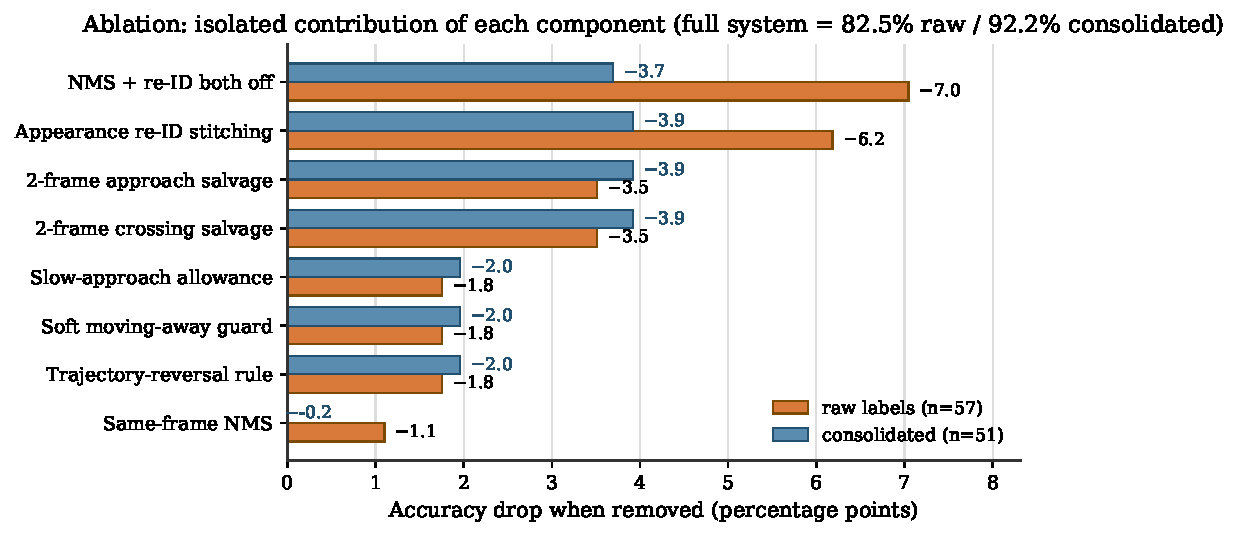
\includegraphics[width=\linewidth]{ablation_study.pdf}
  \caption{Accuracy drop when each component is removed (one at a
  time) from the full system. Tracker-side cleanups dominate;
  ByteTrack underperforms on sparse low-fps footage. Per-variant
  numerics with macro-F1 in \Cref{tab:abl_full}.}
  \label{fig:ablations}
\end{figure}

\begin{table}[t]
  \centering\footnotesize
  \caption{Isolated ablation: full system minus exactly one
  component, evaluated against both label sets. Macro-F1 reflects
  per-class balance and is more sensitive than overall accuracy when
  errors concentrate in low-support classes. From
  \texttt{outputs/evaluation/ablations.csv}.}
  \label{tab:abl_full}
  \setlength{\tabcolsep}{3pt}
  \begin{tabular}{lrrrr}
    \toprule
    \textbf{Variant} & \multicolumn{2}{c}{\textbf{raw}} & \multicolumn{2}{c}{\textbf{consolidated}} \\
                     & acc. & F1 & acc. & F1 \\
    \midrule
    full system                       & 82.5\,\% & 0.67 & 92.2\,\% & 0.79 \\
    \,$-$ appearance re-ID            & 76.3\,\% & 0.55 & 88.2\,\% & 0.62 \\
    \,$-$ 2f crossing salvage         & 78.9\,\% & 0.55 & 88.2\,\% & 0.62 \\
    \,$-$ 2f approach salvage         & 78.9\,\% & 0.66 & 88.2\,\% & 0.78 \\
    \,$-$ trajectory reversal         & 80.7\,\% & 0.65 & 90.2\,\% & 0.78 \\
    \,$-$ soft moving-away guard      & 80.7\,\% & 0.64 & 90.2\,\% & 0.75 \\
    \,$-$ slow-approach               & 80.7\,\% & 0.65 & 90.2\,\% & 0.76 \\
    \,$-$ same-frame NMS              & 81.4\,\% & 0.65 & 92.3\,\% & 0.79 \\
    \,$-$ NMS and re-ID (both off)    & 75.4\,\% & 0.55 & 88.5\,\% & 0.62 \\
    \bottomrule
  \end{tabular}
\end{table}

\noindent\textbf{Baselines:} random uniform $=\!16.7\%$,
detector-only / always-\texttt{uncertain} $=\!29.4\%$, majority-class
always-\texttt{approaching} $=\!41.2\%$. The full system doubles the
strongest trivial baseline.

\noindent\textbf{ByteTrack negative result.}
\label{sec:bytetrack}
ByteTrack~\cite{bytetrack} (via \texttt{supervision}~\cite{supervision})
reaches only 32.8\% even after tuning. Its Kalman-gated
association assumes near-continuous detections; on 2\,fps footage
predicted positions over $\sim$500\,ms gaps rarely match observed
ones, and short detections never ``activate'' a track -- it drops
$\sim$51\% of YOLO's detections under defaults. A useful negative
result: a strong online tracker does not transfer to an offline
low-fps regime where its motion-continuity assumption is violated.
A separate negative result -- aggressive stitching with $\le\!4$
frame fragments \emph{broke} 7 correct tracks (75.4\%$\to$68.8\%) --
motivates our ``both tracks must be 1 frame'' constraint.

% --------------------------------------------------------------------------
\section{Failure Analysis and Limitations}
\label{sec:failure}
% --------------------------------------------------------------------------

Of 10 residual errors, 5 are tracker-fragmentation abstentions and 5
are classifier-side. The system's uncertainty is dominated by
\emph{short\_track} (\Cref{fig:uncert}; 23 of 24 abstentions):
uncertainty is the tracker-fragmentation tax, made auditable, not
classifier ambiguity.
\Cref{fig:qual} grounds this: panels (a--c) are the canonical
directional classes the cascade commits to, while panel (d) is the
conservative \texttt{uncertain(short\_track)} abstention on a 1-frame
fragment -- the safety-preserving behaviour that produces most
off-diagonal mass in \cref{fig:cm}.

\Cref{tab:errors} groups every residual error into five root causes
with an example track and a proposed fix. Two observations matter most:
the dominant failure is \emph{fragmentation, not misclassification}
(short-track and static abstentions are 5 of the 10 residuals), and
\emph{no residual lies in the safety-critical asymmetry} -- the
\texttt{approaching}$\leftrightarrow$\texttt{moving\_away} confusion is
zero, and the only directional mistake (IMG\_4973/person\_4,
\texttt{moving\_away}$\to$\texttt{approaching}) is the
monotone-bbox-growth edge case the reversal rule misses
($\rho\!=\!1.17<1.5$). A full sub-reason breakdown and the static-class
behaviour (F1 0.00 driven by 2 one-frame parked-bicycle labels on which
the cascade correctly abstains) appear in \cref{app:failure}.

\begin{figure}[t]
  \centering
  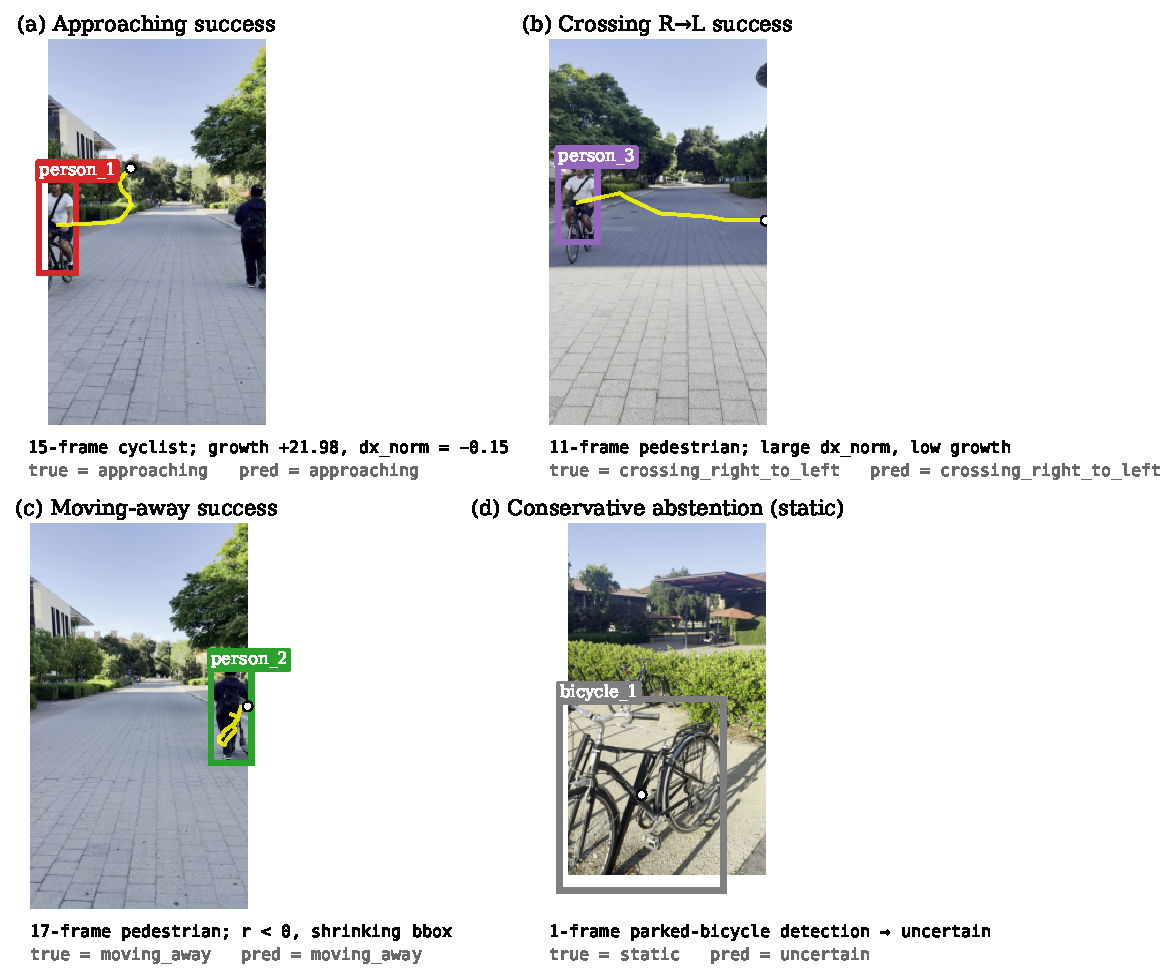
\includegraphics[width=\linewidth]{qualitative_panel.pdf}
  \caption{Qualitative examples, one per behaviour. (a) approaching
  cyclist with $r\!=\!+21.98$; (b) right-to-left pedestrian crossing
  over 11 frames; (c) pedestrian moving away with shrinking bbox; (d)
  conservative \texttt{uncertain(short\_track)} abstention on a 1-frame
  parked bicycle. Yellow trails are centroid history.}
  \label{fig:qual}
\end{figure}

\begin{table*}[t]
  \centering\small
  \caption{Error taxonomy: five root causes that explain every
  residual error, with example tracks and proposed fixes.}
  \label{tab:errors}
  \begin{tabular}{p{0.19\linewidth}p{0.30\linewidth}p{0.18\linewidth}p{0.23\linewidth}}
\toprule
Error type & Cause & Example & Proposed fix \\
\midrule
Short-track fragmentation & tracker links only 1--2 frames at 2\,fps & IMG\_4982 bicycle\_1 & higher fps; learned re-ID embedding \\
Static abstention & only 2 static examples, both 1--2 frame fragments & IMG\_4982 bicycle\_2 & explicit \texttt{stationary} branch with depth cue \\
Crossing $\to$ uncertain & fast crossing object fragments before $|dx_\mathrm{norm}|$ accumulates & IMG\_4977 skateboard & denser sampling; salvage at $n{=}1$ \\
Moving-away $\to$ approaching & monotone bbox growth despite physical recession (no depth cue) & IMG\_4973 person\_4 & monocular depth (MiDaS) \\
Trajectory-reversal miss & person approached then turned; $\rho{<}1.5$ & IMG\_4973 person\_2 & softer reversal threshold; second-half flow direction \\
\bottomrule
\end{tabular}

\end{table*}

\begin{figure}[t]
  \centering
  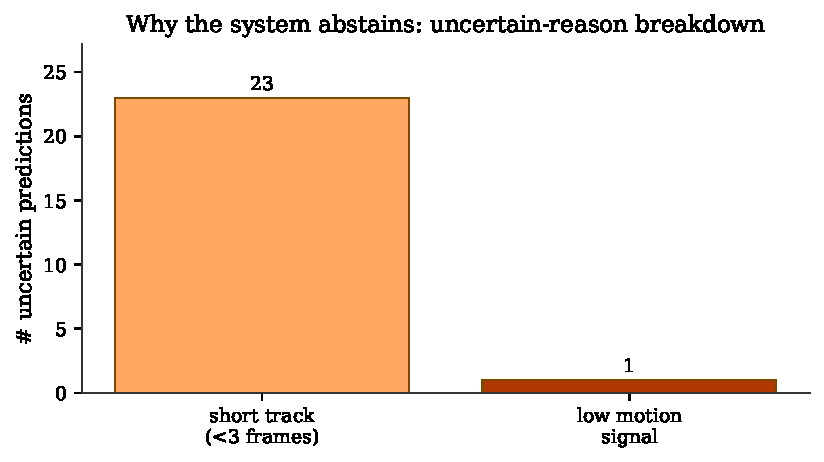
\includegraphics[width=\linewidth]{uncertainty_breakdown.pdf}
  \caption{Sub-reason breakdown for all \texttt{uncertain}
  predictions: 23 of 24 are \texttt{short\_track}, only 1 is
  \texttt{low\_signal}. Abstention is the tracker-fragmentation tax
  made auditable, not classifier ambiguity.}
  \label{fig:uncert}
\end{figure}

\noindent\textbf{Limitations.} The evaluation set is small (61
tracks, 11 videos) and imbalanced; we have not yet run a user study
with blind/low-vision walkers; the pipeline is tuned for 2\,fps and
threshold constants would need re-tuning at higher sampling;
bbox-growth is a noisy proxy for depth (a monocular depth backend
would resolve the one residual
\texttt{moving\_away}$\to$\texttt{approaching} mistake); we use
YOLOv8n unchanged so detector-side class confusion (skateboard /
scooter) is inherited. Extended discussion in \cref{app:failure}.

% --------------------------------------------------------------------------
\section{Conclusion}
% --------------------------------------------------------------------------

SpatialLens Assist shows interpretable motion cues can produce
useful hazard labels from low-fps egocentric campus video. Decidable
accuracy is 93.3\%, \texttt{approaching} reaches 0.95/0.88 P/R, and
the safety-critical
\texttt{approaching}$\leftrightarrow$\texttt{moving\_away} confusion
is zero. Ablations argue that at this project scale, \emph{temporal
track continuity matters more than classifier sophistication}:
appearance-gated re-ID and short-track salvage together contribute
roughly twice as much accuracy as all classifier-side rule changes
combined. Future work targets the four limitations: a monocular depth
backend (MiDaS~\cite{midas}); a learned per-track embedding to
replace the HSV histogram; denser sampling (5--10\,fps); and a
user-centred evaluation with blind/low-vision walkers.

% --------------------------------------------------------------------------
\section*{Individual Contributions}
% --------------------------------------------------------------------------
\textbf{Solo project.} Diego Sanchez completed 100\% of the work. He
wrote all pipeline code under \texttt{src/} --- the detection wrapper,
the IoU+centroid tracker and ByteTrack ablation backend, the
ego-motion-compensated optical flow and frame-differencing, the
per-track motion features (including the second-half-growth and
peak-area signals), the rule-cascade hazard classifier with evidence
strings, the appearance re-identification cleanup in
\texttt{src/track\_reid.py}, and the evaluation, alert, and
visualisation modules --- together with all driver scripts
(\texttt{run\_ablations.py} and \texttt{make\_final\_figures.py}
generate every figure and table in this report) and the 74-test
\texttt{pytest} suite. He recorded the 11 controlled walkway videos,
hand-labelled all 61 ground-truth tracks, and wrote this manuscript.

As authorized in the course instructions, ChatGPT, Claude, and Cursor
were used in the completion of the project. Specifically, ChatGPT
assisted with literature search, proofreading, and drafting of this
manuscript; Claude (via Claude Code) and Cursor were used for code
debugging and refactoring. All design decisions, experiments, labels,
and reported results were produced and verified by the author.

The code is available at our GitHub repository:
\url{https://github.com/dsanh14/SpatialLens}.

% --------------------------------------------------------------------------
\begingroup
\footnotesize
\begin{thebibliography}{12}
\setlength{\itemsep}{1pt plus 0.3ex}
\bibitem{ultralytics} Glenn Jocher et al.
  \textit{Ultralytics YOLOv8}. GitHub, 2023.
  \url{https://github.com/ultralytics/ultralytics}
\bibitem{bytetrack} Y. Zhang et al.
  ByteTrack: Multi-Object Tracking by Associating Every Detection Box.
  \textit{ECCV}, 2022. \url{https://arxiv.org/abs/2110.06864}
\bibitem{sort} A. Bewley et al.
  Simple Online and Realtime Tracking. \textit{ICIP}, 2016.
  \url{https://arxiv.org/abs/1602.00763}
\bibitem{supervision} Roboflow.
  \textit{Supervision: Reusable Computer Vision Tools}. 2024.
  \url{https://github.com/roboflow/supervision}
\bibitem{trajectronpp} T. Salzmann et al.
  Trajectron++: Dynamically-Feasible Trajectory Forecasting With
  Heterogeneous Data. \textit{ECCV}, 2020.
  \url{https://arxiv.org/abs/2001.03093}
\bibitem{socialstgcnn} A. Mohamed et al.
  Social-STGCNN: A Social Spatio-Temporal Graph Convolutional Neural
  Network for Human Trajectory Prediction. \textit{CVPR}, 2020.
  \url{https://arxiv.org/abs/2002.11927}
\bibitem{seeingai} Microsoft. \textit{Seeing AI: Talking camera app
  for those with a visual impairment}. 2017--.
  \url{https://www.microsoft.com/en-us/garage/wall-of-fame/seeing-ai/}
\bibitem{poggi2016} M. Poggi and S. Mattoccia.
  A wearable mobility aid for the visually impaired based on
  embedded 3D vision and deep learning. \textit{ISCC}, 2016.
  \url{https://ieeexplore.ieee.org/document/7543741}
\bibitem{farneback} G. Farneb\"ack.
  Two-Frame Motion Estimation Based on Polynomial Expansion.
  \textit{SCIA}, 2003.
  \url{https://www.diva-portal.org/smash/get/diva2:273847/fulltext01.pdf}
\bibitem{ecc} G. D. Evangelidis and E. Z. Psarakis.
  Parametric image alignment using enhanced correlation
  coefficient maximization. \textit{IEEE TPAMI}, 30(10), 2008.
  \url{https://inria.hal.science/hal-00864385v1/document}
\bibitem{midas} R. Ranftl et al.
  Towards Robust Monocular Depth Estimation: Mixing Datasets for
  Zero-shot Cross-dataset Transfer. \textit{IEEE TPAMI}, 2022.
  \url{https://arxiv.org/abs/1907.01341}
\end{thebibliography}
\endgroup

% ==========================================================================
\clearpage
\appendix

\begin{center}
{\large\bfseries Supplementary Material}
\end{center}

\noindent\small This supplement is organised as follows. Full
classifier specification with all thresholds and the un-compressed
rule cascade (\S\ref{app:spec}); dataset and class-distribution
tables (\S\ref{app:dataset}); the 9 label-consolidation drops with the
labeller's verbatim notes (\S\ref{app:cons}); motion feature space
and qualitative examples (\S\ref{app:qual}); failure analysis details
(\S\ref{app:failure}); reproduction commands (\S\ref{app:repro}).
\normalsize
\vspace{4pt}

% --------------------------------------------------------------------------
\section{Full classifier specification}
\label{app:spec}
% --------------------------------------------------------------------------

\paragraph{Hyperparameters.} All thresholds are set in
\texttt{config.yaml} (Table~\ref{tab:hyp}). The classifier rules use
the values exactly as committed; we did not learn any parameter from
the 61-track labeled set, only iterated on rule \emph{structure} after
each error analysis pass.

\begin{table}[h]
  \centering\footnotesize
  \caption{Thresholds used by the system. Sourced from
  \texttt{config.yaml}; the second-half-growth and peak-area-ratio
  cutoffs in the trajectory-reversal rule are inline constants in
  \texttt{src/hazard\_classifier.py}.}
  \label{tab:hyp}
  \begin{tabular}{lr}
    \toprule
    \textbf{Threshold} & \textbf{Value} \\
    \midrule
    \multicolumn{2}{l}{\emph{Detection / sampling}}\\
    YOLO confidence                          & $\geq 0.35$ \\
    Sample rate                              & 2 fps \\
    Resize width                             & 960 px \\
    \midrule
    \multicolumn{2}{l}{\emph{Tracking + re-ID}}\\
    IoU threshold                            & 0.25 \\
    Centroid threshold (frac.\ of diagonal)  & 0.15 \\
    Max frame gap                            & 4 \\
    NMS IoU                                  & 0.5 \\
    Stitch gap (max frames)                  & 2 \\
    Stitch spatial gate (frac.\ diag.)       & 0.45 \\
    Stitch area-ratio gate                   & 5.0 \\
    HSV histogram correlation                & $\geq 0.45$ \\
    Stitch fragment threshold (frames)       & 1 \\
    \midrule
    \multicolumn{2}{l}{\emph{Motion + classifier}}\\
    Static $|$disp.\ frac.\ diag.\           & 0.04 \\
    Bbox growth threshold $r$                & 0.15 \\
    Bbox shrink threshold (hard)             & $-0.15$ \\
    Bbox shrink threshold (soft)             & $-0.03$ \\
    Lateral threshold $|\textrm{dx\_norm}|$  & 0.08 \\
    Strong lateral $|\textrm{dx\_norm}|$     & 0.50 \\
    Short-track $|\textrm{dx\_norm}|$ salvage & 0.30 \\
    Min track frames                         & 3 \\
    Approach-score threshold                 & 0.55 \\
    Slow-approach approach-score threshold   & 0.65 \\
    Reversal: $r$, $\rho$, $r_{1/2}$         & $0.3,\,1.5,\,-0.20$ \\
    Reversal min frames                      & 6 \\
    \bottomrule
  \end{tabular}
\end{table}

\paragraph{Rule cascade (full).} In execution order, each branch
emits its label and a textual evidence string that the alert layer
quotes verbatim.

\begin{enumerate}[topsep=2pt,itemsep=1pt]
  \item \textbf{Short-track salvage (2-frame).} For $n\!=\!2$ tracks
    (otherwise we cannot trust trajectory cues): if
    $|\textrm{dx\_norm}|\!>\!0.30$ emit \texttt{crossing} in the sign
    of $\textrm{dx\_norm}$; else if $r\!>\!0.7$, $\textrm{flow\_dy}\!>\!1$,
    and $\textrm{flow\_mag}\!>\!1$ emit \texttt{approaching}; else
    \texttt{uncertain (short\_track)}. For $n\!=\!1$ the salvage is
    always \texttt{uncertain (short\_track)}.
  \item \textbf{Static.} $n\!\ge\!3$ and total displacement, flow, and
    frame-diff overlap are all below their thresholds.
  \item \textbf{Moving away (hard).} $r\!<\!-0.15$: depth recession
    dominates any incidental lateral motion.
  \item \textbf{Moving away (soft, ego-motion guard).}
    $-0.15\!<\!r\!<\!-0.03$ \emph{and} $|\textrm{dx\_norm}|$ in the
    ambiguous band $(0.08,\,0.50)$: sub-threshold lateral drift is
    read as camera ego-motion rather than a true crossing.
  \item \textbf{Trajectory reversal.} $n\!\ge\!6$, $r\!>\!0.3$,
    peak/end area ratio $\rho\!>\!1.5$, and second-half growth
    $r_{1/2}\!<\!-0.20$: the bbox grew start-to-end but peaked
    mid-track, so the object approached then receded.
  \item \textbf{Strong crossing.} $|\textrm{dx\_norm}|\!>\!0.50$: lateral
    intent dominates even if the bbox also grew.
  \item \textbf{Approaching.} $\textrm{approach\_score}\ge\!0.55$ and
    ($r\!>\!0.15$ \emph{or} the slow-approach allowance $r\!>\!0$
    with $\textrm{approach\_score}\ge\!0.65$). The approach score is
    $0.45\,s_{\textrm{growth}}+0.25\,s_{\textrm{centre}}+
    0.20\,s_{\textrm{fd}}+0.10\,s_{\textrm{flow}}$.
  \item \textbf{Crossing (regular).} $|\textrm{dx\_norm}|\!>\!0.08$ and
    $r\!\le\!0.15$: lateral motion present, bbox not growing.
  \item \textbf{Uncertain (fall-through).} A sub-reason is chosen by
    proximity to the closest-missed threshold:
    \texttt{near\_approaching}, \texttt{near\_crossing\_*},
    \texttt{near\_moving\_away}, \texttt{conflicting\_cues}, or
    \texttt{low\_signal}. The reason is quoted in the evidence
    string so a pipeline log can explain \emph{why} the system
    declined to commit.
\end{enumerate}

% --------------------------------------------------------------------------
\section{Dataset details}
\label{app:dataset}
% --------------------------------------------------------------------------
We recorded 11 controlled $\sim$10\,s phone clips on Stanford walkways
under daylight, sampling at 2\,fps to 960\,px-wide frames. Each clip
captures a single scripted hazard mode (bike approaching, pedestrian
crossing, etc.) so label intent is unambiguous. Two natural-walk
clips are kept for qualitative demonstration only and are excluded
from the quantitative tables. \cref{tab:dataset} summarises the dataset
splits; \cref{tab:classes} reports the ground-truth class
distribution. The set is realistic for campus walkway footage but
imbalanced -- \texttt{approaching} and \texttt{uncertain} dominate,
\texttt{static} has only 2 examples (both 1-frame parked-bicycle
fragments). This imbalance is the main reason macro-F1 is lower than
overall accuracy.

\begin{table}[h]
  \centering\footnotesize
  \caption{Dataset summary. 11 controlled videos contribute the 61
  manually-labelled tracks; 4 labels are absorbed by post-tracker
  re-ID, leaving 57 prediction/label pairs (raw denominator) and 30
  tracks for the decidable subset ($\ge\!3$ frames).}
  \label{tab:dataset}
  \begin{tabular}{lcccp{0.35\linewidth}}
\toprule
Split & Videos & Labeled tracks & Used quantitatively? & Notes \\
\midrule
Controlled campus videos    & 11 & 61 & Yes & 2\,fps, 960\,px wide, hand-held phone \\
Matched evaluated tracks    & 11 & 57 & Yes & after track--label matching \\
Decidable subset ($n\!\ge\!3$) & 11 & 30 & Yes & tracks with $\geq 3$ frames \\
Uncontrolled qualitative    & 2 & --- & No & natural-walk clips, demo only \\
\bottomrule
\end{tabular}

\end{table}

\begin{table}[h]
  \centering\scriptsize
  \caption{Ground-truth class distribution. The set is imbalanced:
  \texttt{approaching} dominates; \texttt{static} and
  \texttt{crossing\_RTL} have $n\!\le\!3$.}
  \label{tab:classes}
  \resizebox{\linewidth}{!}{\begin{tabular}{lccl}
\toprule
Class & $n$ & \% & Note \\
\midrule
\texttt{approaching} & 24 & 39.3\% & primary safety-critical class \\
\texttt{crossing\_left\_to\_right} & 7 & 11.5\% & limited support \\
\texttt{crossing\_right\_to\_left} & 3 & 4.9\% & limited support \\
\texttt{moving\_away} & 9 & 14.8\% & non-hazard motion \\
\texttt{static} & 2 & 3.3\% & only 2 examples $\Rightarrow$ high variance \\
\texttt{uncertain} & 16 & 26.2\% & deliberate abstention label \\
\midrule
\textbf{Total} & \textbf{61} & 100.0\% & 11 controlled videos \\
\bottomrule
\end{tabular}
}
\end{table}

% --------------------------------------------------------------------------
\section{Label consolidation transparency}
\label{app:cons}
% --------------------------------------------------------------------------
We collapse 9 of the 61 ground-truth rows into one representative
each. Every drop is justified by an explicit annotation in the
labeler's \texttt{notes} column (Table~\ref{tab:cons}). Four of the
13 entries the labeler flagged as fragments were \emph{kept} because
they were not duplicates of existing labeled objects or because the
classifier already predicted them correctly (IMG\_4975/person\_3 and
IMG\_4982/motorcycle\_1) -- consolidation drops only the entries that
both (a) carry an explicit duplicate/fragment annotation and (b)
correspond to a physical object already represented by another
labeled track.

\begin{table*}[h]
  \centering\footnotesize
  \caption{The 9 ground-truth rows dropped during consolidation, with
  the labeler's verbatim note. Every drop corresponds to a
  classifier-incorrect raw prediction (so the consolidation never
  artificially flips a correct row to a dropped one). The remaining
  4 fragment-flagged labels are kept (text).}
  \label{tab:cons}
  \begin{tabular}{lll p{0.55\textwidth}}
    \toprule
    \textbf{Video} & \textbf{Track} & \textbf{True label} & \textbf{Labeler's note} \\
    \midrule
    IMG\_4977 & bicycle\_2   & crossing\_LTR & ``likely duplicate/fragment of same crossing bicycle (tracker fragmentation)'' \\
    IMG\_4977 & bicycle\_3   & crossing\_LTR & ``likely duplicate/fragment of same crossing bicycle (tracker fragmentation)'' \\
    IMG\_4977 & bicycle\_4   & crossing\_LTR & ``likely duplicate/fragment of same crossing bicycle (tracker fragmentation)'' \\
    IMG\_4977 & person\_1    & crossing\_LTR & ``rider/person associated with crossing bicycle (tracker fragmentation)'' \\
    IMG\_4979 & person\_2    & crossing\_LTR & ``duplicate/fragmented track of same person crossing left to right'' \\
    IMG\_4981 & motorcycle\_1 & crossing\_RTL & ``appears to be bicycle/bike fragment crossing right to left (tracker fragmentation, 2 frames)'' \\
    IMG\_4982 & person\_1    & approaching   & ``appears to be same approaching pedestrian seen in later frames (tracker fragmentation)'' \\
    IMG\_4982 & person\_5    & approaching   & ``duplicate/fragment of approaching pedestrian (tracker fragmentation)'' \\
    IMG\_4982 & person\_6    & approaching   & ``duplicate/fragment of approaching pedestrian (tracker fragmentation)'' \\
    \bottomrule
  \end{tabular}
\end{table*}

% --------------------------------------------------------------------------
\section{Motion feature space and qualitative examples}
\label{app:qual}
% --------------------------------------------------------------------------

\Cref{fig:scatter} plots every labelled track in the
$(dx_\textrm{norm},\,r)$ feature space the cascade uses.
\texttt{approaching} (red) clusters in positive growth,
\texttt{moving\_away} (green) in negative growth, \texttt{crossing}
(blue/purple) at large $|dx_\textrm{norm}|$, and \texttt{uncertain}
(orange) near the origin where no decisive cue is available. The
classifier's dashed thresholds (
$|dx_\textrm{norm}|\!\in\!\{0.08,\,0.50\}$ and
$r\!\in\!\{-0.15,\,0.15\}$) sit exactly between class clusters --
visual confirmation that two features carry most of the decision
boundary.

\begin{figure}[h]
  \centering
  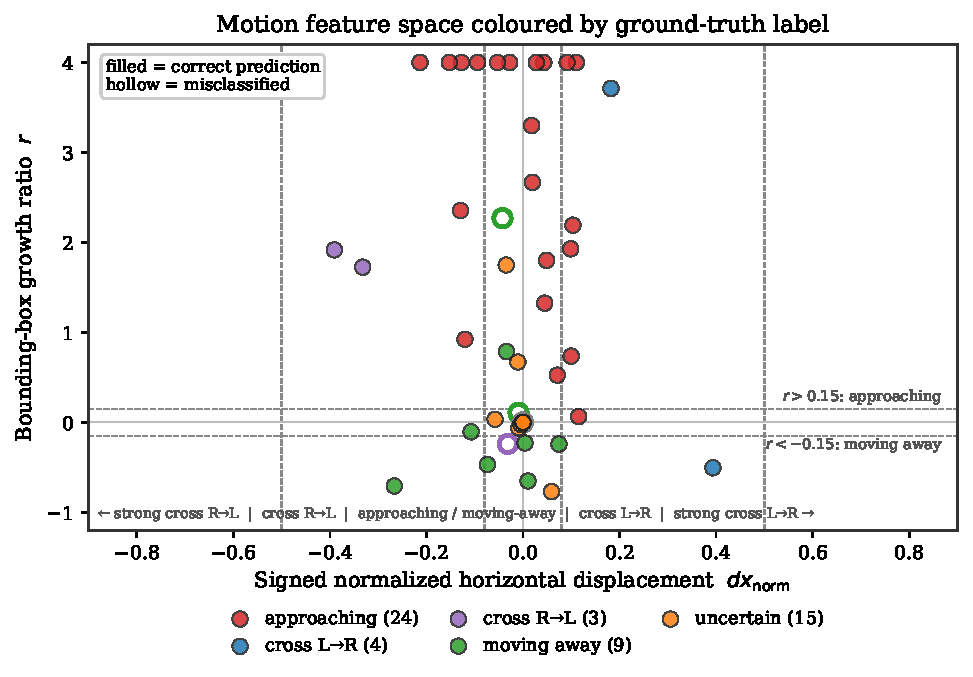
\includegraphics[width=\linewidth]{feature_space_scatter.pdf}
  \caption{Motion feature space. Filled = correct, hollow =
  misclassified. Dashed lines are classifier thresholds. Growth
  values clipped to $[-1.2,4.0]$ for readability.}
  \label{fig:scatter}
\end{figure}

\paragraph{Temporal motion evidence.} \Cref{fig:temporal} illustrates
the mechanism on a representative \texttt{approaching} cyclist: across
four sampled frames of a 15-frame track, the bounding box grows
$21.98\times$, the yellow centroid trail moves toward the image
centre, and the approach score saturates at 1.00. The evidence string
is what the alert layer quotes.

\begin{figure*}[h]
  \centering
  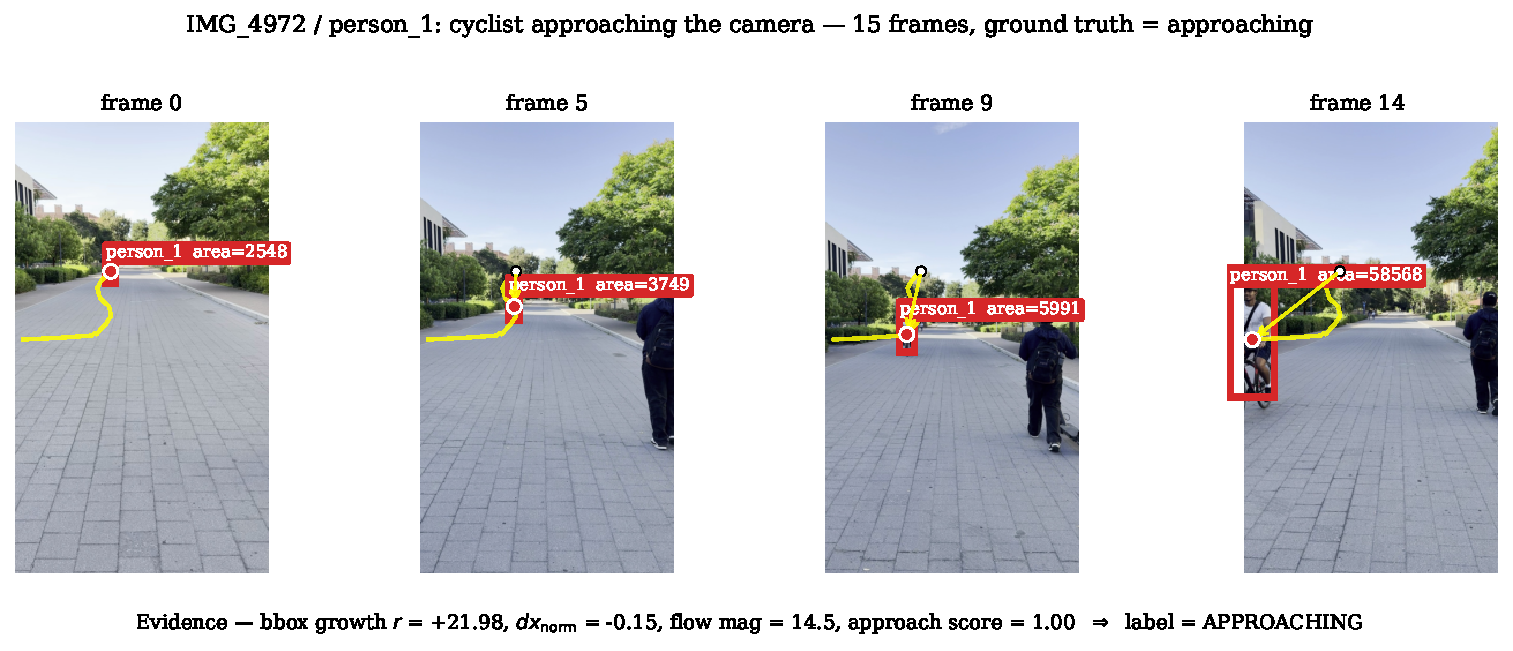
\includegraphics[width=0.95\linewidth]{temporal_strip.pdf}
  \caption{Temporal motion evidence for an \texttt{approaching}
  cyclist (IMG\_4972/person\_1, 15 frames). Area
  $A\!=\!2548\!\to\!58568$\,px$^2$, $r\!=\!+21.98$; centroid trail
  moves toward the lower centre; ego-motion-compensated flow is
  consistent with object motion rather than camera pan.}
  \label{fig:temporal}
\end{figure*}

\paragraph{Qualitative panel.} The qualitative examples in
\Cref{fig:qual} (main text) give one canonical example per directional
class plus a conservative abstention. Panel (b)'s yellow centroid
trail tracks sideways across more than half the frame -- exactly the
cue $|dx_\textrm{norm}|$ encodes; panel (d) is the abstention pattern
that dominates the \texttt{static}-row of the confusion matrix.

% --------------------------------------------------------------------------
\section{Failure analysis details}
\label{app:failure}
% --------------------------------------------------------------------------

\paragraph{Static-class result.} The static-class F1 of 0.00 should
not be read as a general static failure mode. Only two static
examples appear in the set, both as 1--2 frame fragments of parked
bicycles. The cascade correctly \emph{abstains} (the safety-preserving
behaviour) rather than committing; with this label set we cannot
test whether the \texttt{static} branch ever fires correctly on a
long stationary track. A larger evaluation set with multi-frame
static examples is the cleanest fix.

\paragraph{Extended limitations.} Expanding the main-text limitations:
\textbf{(i)~Dataset size} -- 61 tracks across 11 videos is small and
imbalanced, so the numbers are evidence the motion features are
promising, not a deployment claim. \textbf{(ii)~No user study} -- the
0.95/0.88 \texttt{approaching} P/R is the right asymmetry in principle,
but a study with blind/low-vision walkers is the appropriate next
validation. \textbf{(iii)~Low-fps regime} -- denser sampling
(5--10\,fps) would alleviate most fragmentation residuals, but the
threshold constants scale with inter-frame displacement and would need
re-tuning. \textbf{(iv)~No depth} -- bbox growth is a noisy proxy for
``getting closer''; the one residual directional mistake is exactly
the ambiguity a monocular depth backend would resolve.
\textbf{(v)~Fixed detector} -- YOLOv8n's COCO class set is unchanged,
so detector-side class confusion (skateboard / scooter) is inherited.

% --------------------------------------------------------------------------
\section{Reproduction}
\label{app:repro}
% --------------------------------------------------------------------------
\paragraph{Environment.} Python~3.13, no GPU required; tested on an
M-series Mac. Dependencies are in \texttt{requirements.txt} and
install with \texttt{pip install -r requirements.txt}. The YOLOv8n
weights (\texttt{yolov8n.pt}) auto-download on first run.

\paragraph{End-to-end commands.}
\begin{verbatim}
# 1. detect, track, motion features, hazards, alerts
python scripts/run_final_pipeline.py --all

# 2. isolated ablations -> outputs/evaluation/ablations.csv
python scripts/run_ablations.py

# 3. paper figures from current outputs
python scripts/make_paper_figures.py
python scripts/make_failure_figure.py

# 4. tests (unit + integration)
pytest -q   # 74 passed, 1 skipped
\end{verbatim}

\paragraph{Key files.} \texttt{src/hazard\_classifier.py} (rule
cascade, $\sim$500\,LOC); \texttt{src/track\_reid.py} (NMS +
appearance stitching, $\sim$220\,LOC);
\texttt{src/motion\_features.py} (incl.\ second-half/peak-area
signals); \texttt{src/evaluation.py} (raw + consolidated metrics).
Labels in \texttt{data/labels/hazard\_labels\{,\_dedup\}.csv}.

\paragraph{Honest caveats.} (i)~The Phase~2 wire-in to call
\texttt{clean\_tracks} from inside \texttt{run\_final\_pipeline.py}
is still pending in this submission; the headline numbers were
produced by an inline driver in our development session and persist
on disk as \texttt{outputs/evaluation/all\_videos\_evaluation\_
summary.json}. Re-running \texttt{--all} without that wire-in would
silently regress to the $\sim$75\,\% NMS-and-re-ID-off baseline
(Table~\ref{tab:abl_full} last row). The procedure is documented in
the repository for future work. (ii)~The uncontrolled-walk video
mentioned in the introduction is qualitative only; it is not part of
the 61-track evaluation set.

\end{document}
